\begin{itemize}
	\item \hypertarget{veichle:Death_Rogumer}{\textbf{Death Rogumer:}}
	An Aerial battleship made for the Maverick Hunter's air cavalry. Originally made in order to hold down reploid rebellions, Sigma converted it as a fortress 
	for his army, entrusting the command to former leader of 7th Aribone unit, Storm Eagle~\cite{wayback:X_resources}.
	\begin{figure}[htp]
		\centering
		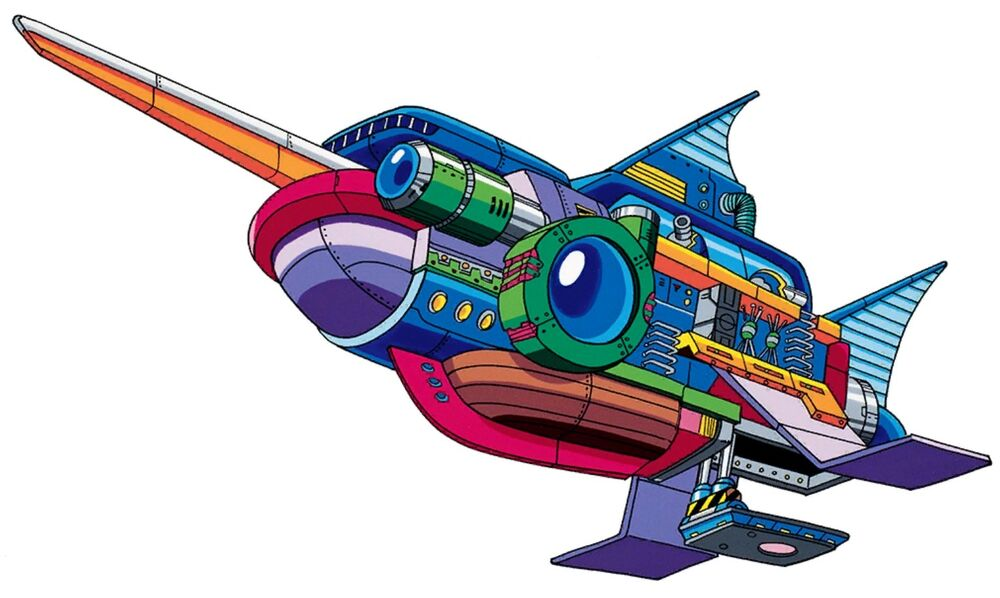
\includegraphics[width=\linewidth]{figures/X1/Storm_eagle/DeathRogumer.jpg}
		\caption{Death Rogumer}
	\end{figure}
	\item \hypertarget{veichle:Ride_Armor}{\textbf{Ride Armor:}}
	Ride Armors are mechas similar to tanks with attached hands and feet. Originally these machines were made intended to be used in engineering~\cite{wayback:X_resources}, but were latter used also for fighting, as they greatly increase the power of their user due being able to dash, walk over spikes, deliver powerful attacks and receive damage in place of 
	their pilot. Starting from these base version many other will be created, focused more on combat power. Vile himself uses two modified Ride Armors in his confrontation with X, although both of them were destroyed by Zero.
	\begin{figure}[htp]
		\centering
		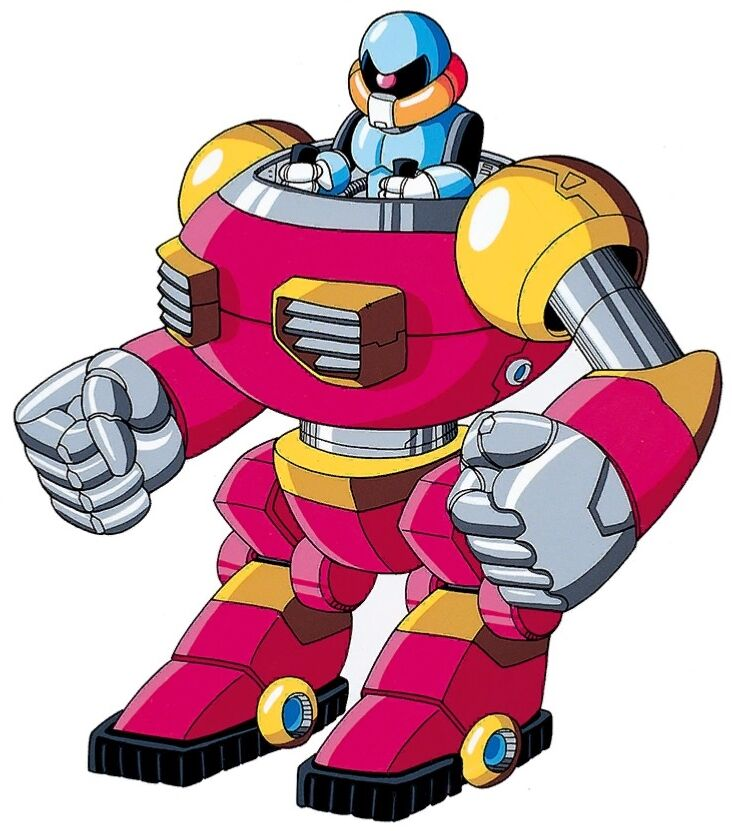
\includegraphics[width=0.5\linewidth]{figures/X1/Enemies/ArmorSoldier.jpg}
		\caption{Ride Armor 's artwork (with pilot)}
	\end{figure}
	
	\item \hypertarget{veichle:Ride_Armor_Rabbit}{\textbf{Ride Armor EG-2 custom "\textit{Rabbit}":}}


	\item \hypertarget{veichle:Ride_Chaser_Cheval}{\textbf{Ride Chaser ADU-T400 turbo "\textit{Cheval}": }}	
\end{itemize}